ネットワークの境界において,必要のない通信を遮断するファイアウォールやパ
ケットフィルタと呼ばれる機能を有効にすることは重要である.また,それらに
よって外部の機器への通信を制限される内部の機器のために NAT という機能によ
る通信の仲介を行わせることがある.NAT は内部から外部に対する通信を制御す
るだけでなく,内部ネットワークのセキュリティ確保にも役立つ.

\section{ネットワークセキュリティ}
これまで,TCP/IP によるネットワークの構築を行い,多くのネットワークサービスを立ち上げ,
利用者の利便性の向上につながるネットワークシステムの構築を行ってきた.

ルーティングを行い TCP/IP の接続性を向上させ,DNS, Web, 電子メールシステ
ムを構築することで,インターネットを通して世界中から接続可能なネットワー
クサービスの構築を行った.同時に,ファイル転送・ファイル共有などの仕組み
を構築し,情報のやりとりの利便性も向上した.

これまでのネットワークサービスの構築においても,端末ごとのOSのアップデー
トやウイルス対策,サービスごとのアクセス制限など,個々のコンピュータやサー
ビス単位でのセキュリティの設定を行ってきた.

大規模ネットワークの管理を行う場合でも,全ての端末に対して常に万全のセキュ
リティを求めることは重要であるが,セキュリティホール1つからネットワーク
の端末全体の危険が誘発されるような事態も起こり得ることや,多重保護の観点
からもネットワーク単位でのセキュリティも重要となる.

このような目的でネットワーク全体の保護に用いられるセキュリティ技術として,
ファイアウォール(防火壁)がある.ファイアウォールは,ネットワークの入口
で,セキュリティ上好ましくない通信や,不必要な通信を遮断し,アクセス制限
を行う.ファイアウォールには,ネットワーク外部からの攻撃などを遮断する意
図の他,ネットワーク内部からの外部へ向けての攻撃などを防ぐ意図など
もある.具体的には,外部からの攻撃を誘発したり助けたりするような内部から
外部へ向けてのアクセスや,ウイルスなどに感染した内部ホストからの外部への
攻撃をネットワークの入口で防ぐ意図がある.

\subsection{ファイアウォール}
%本課題では,ファイアウォールの構築を行う.
ファイアウォールは,ネットワークのアクセスを選別し必要のあるアクセスの
みを通過させ,そうでないアクセスを遮断する技術である.

ファイアウォールを用いることによりネットワーク・セキュリティを向上させ
ることができる.しかし,ファイアウォールを構築するだけですべての攻撃を
防ぐことはできない.例えば,ファイアウォールではメールに添付されている
コンピュータウィルスを除去することはできない.また,Web サーバに対して
行なわれる正常な http アクセスを装った DDoS 攻撃\footnote{distibuted
  denial of service の略.複数の拠点から標的のサーバへ一斉に DoS 攻撃を
  仕掛ける.}には対処できない.そして,新しい脅威に対しては,防御できな
い場合も十分に考えられる.そのため,ファイアウォールの運用においては必
ず他のセキュリティ技術と組み合わせることが必要である.

%\subsection*{ファイアウォールの種類}
ファイアウォールには,大きく分けて次の二種類がある.これは,パケット処
理を行うネットワークレイヤーによる違いである.

\subsection*{パケットフィルタリングファイアウォール}
図\ref{fig:06:pf}に示すように,内部ネットワークと外部ネットワークの境界
に位置するルータにおいて,パケットフィルタリングルールに従って,二つのネッ
トワーク間でのパケット転送を制御する.宛先IPアドレス・送信元IPアドレス,
プロトコルの種類やポート番号等,IP・TCP・UDP ヘッダの情報に基づく制御
を行う.パケット毎に処理を行い,データの塊や接続状態(セッションの状態)などは基本的に関知しない.ただし,近年の高機能ファイアウォール専用製品ではステートフルインスペクションと呼ばれ
るステート(=TCPの状態,Established か否かや Syn,Fin なども条件に加える)
を加味したパケットフィルタや,HTTPやSMTPのコンテンツ,ウイルス,攻撃検出もある程度も行うディープパケットインスペクションなども一般的になってきている.このような機器では,処理が複雑になり状態を記憶する必要もあり,性能を出すためにはメモリや処理性能が求められる(遅くとも良ければ,サーバでも可能).


\subsection*{アプリケーションゲートウェイファイアウォール}
図\ref{fig:06:ag}に示すように,アプリケーション層において,定められたルー
ルに従ってパケットを中継する,あるいは拒否するファイアウォールである.こ
のため,アプリケーションごとの制御や,データ単位での制御,ユーザ単位での
制御が行え,パケットフィルタリングよりもきめ細かい制御が可能となる.実際
の接続を,このゲートウェイが代行することになるので,プロキシ(Proxy:代理)
とも言う.

DNSのキャッシュサービス,電子メールの SMTP サービスも,クライアントの要
求をサーバが代行して行うという点で,一種のアプリケーションゲートウェイで
ある.

近年では,パケットフィルタとアプリケーションゲートウェイを組み合わせるパ
ターンが多くなっている\footnote{実際には,内側(trust側),外側(untrust側)
をパケットフィルタで分離し,さらに,内側と外側の両方からアクセス可能な
DMZ (非武装地帯) を作成して,アプリケーショ
ンゲートウェイとなるサーバをここに設置する.}.ここでは,パケットフィル
タで内側 (trust側) と外側 (untrust側) の通信を完全に遮断し,サーバだけは
外部との必要な通信を許可し,内側の PC からは,アプリケーションゲートウェイやメールサー
ビス・DNS サービスを経由して外側のサービスを受信できるようにする.

このように,LAN の一部を完全に外部から遮断する形は,安全性が高いが,利便性の面で利用者が不便になる点もある.

\begin{figure}[h]
 \begin{center}
  \resizebox{!}{4cm}{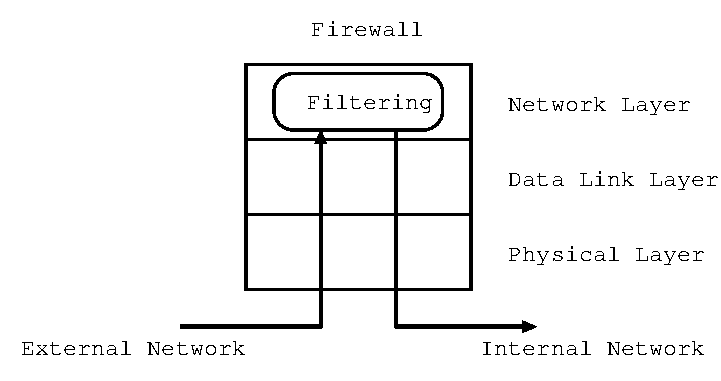
\includegraphics{./06_firewall_appgw/fw1.eps}}
  \caption{パケットフィルタリング}
  \label{fig:06:pf}
 \end{center}
\end{figure}

\begin{figure}[h]
  \begin{center}
   \resizebox{!}{4cm}{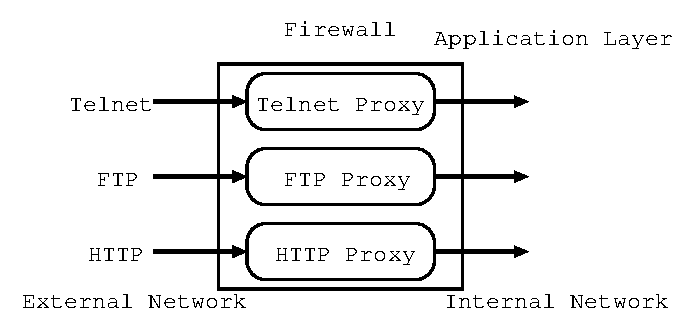
\includegraphics{./06_firewall_appgw/fw2.eps}}
  \caption{アプリケーションゲートウェイ}
  \label{fig:06:ag}
 \end{center}
\end{figure}

\subsection{NAT}

Network Address Translation (NAT: ネットワークアドレス変換) は,IP パケッ
トの送信元アドレス,宛先アドレスの一方または双方を書き換えて転送するもの
である.狭い意味で NAT と言う場合,IP アドレスのみの書き換えを指すことが
ある.

UDPデータグラム,TCPセグメントの送信元ポート番号,宛先ポート番号も同時に
変換する場合もあり,これを,NAPT(Network Address Port Translation), PAT
(Port Address Translation: Cisco社が主に呼称), IP Masquerade (IPマスカレー
ド: Linux システムが主に呼称) と呼ぶ.あるいは,NAPT を 単に NAT と呼称
する場合も多く,むしろ現在は,アドレス加えてポート番号も変関する場合がほ
とんであるので,NAT = NAPT と考えてもほとんど差し支えない.

内側から外側ネットワークへの接続に NAT を用いると送信元 IP アドレスなど
のネットワーク情報が置き換わるため,下記のような利点があり,よく利用され
る.

\begin{itemize}
 \item 1つの IP アドレスで複数のコンピュータをインターネットへ接続する.
 \item 外側から内側への接続を制限し,かつ,内側のネットワーク情報を隠蔽
       することで,簡易的なファイアウォールとしてセキュリティを向上させ
       る.
 \item NAT の外側からは,1台のコンピュータとして見せることができるため,
       ある LAN をルーティングプロトコルやルーティング設定を行
       うことなく,別の LAN に接続することができる.家庭内 LAN のインター
       ネットへの接続は,この例である.
\end{itemize}

なお,家庭用のインターネット接続用ブロードバンドルータや無線LANルータと
呼ばれる製品は,NAPT を行うものである(静的ルーティングや RIP による L3 
ルーティングは一部サポートされているが,ほとんど用いることはない).この
ため,ネットワーク技術とは異なる場面で,単にルータといった場合に,NAPT 
を指すこともしばしばあるので注意する(ネットワーク技術に関する話を行う場
では,NAPTの意味でルータの語を用いることはまれである).

\subsection*{NATの種類}

\begin{description}
 \item[スタティックNAT] \ \\
            狭い意味での NAT であり,IP アドレスを単順に置き
	    換える.置き換える前の IP アドレスと,置き換え後の IP アドレ
	    スが一対一に対応し,常にその対応通りに置き換わる場合をスタ
	    ティック(静的) NAT と呼ぶ.内側からも外側からも,また,すべ
	    てのポート番号の UDP/TCP,あるはそれ以外のすべての IP パケッ
	    トについて変換を行い,常にパケットを転送することができるので,
	    サーバを公開する際などに用いることができる.欠点として,セキュ
	    リティは,NAT を行わずに直接外側ネットワークに接続する場合と
	    変わらないことから,十分なセキュリティ対策を行わないと NAT 
	    内側ネットワークが危険になることや,外側の IP アドレスを常に
	    1台につき1つずつ必要であることが挙げられる.すなわち対応づけ
	    られたコンピュータ以外は,その IP アドレスを用いることはでき
	    ない.
 \item[スタティックNAPT (PAT)] \ \\
            置き換える前の IP アドレスおよびポート番号と,置き換え後の 
	    IP アドレスおよびポート番号の対を,あらかじめルータに静的に
	    設定しておくものである.すなわち,NATテーブルの変換エントリ
	    をあらかじめ作成しておく.事項で説明するオーバーロードあり動
	    的 NATは,内側から外側へのアクセスがあると,その時に動的に
            NAT エントリが NAT テーブルに作成されるが,静的 NAT ではあら
            かじめ作成しておくため,外側から内側へのアクセス要求にも,
            変換および転送ができる.このため,この後に説明するポートフォ
            ワーディング(ポート転送)に用いられ,サーバ公開(NAT内部に置い
            たサーバを外部からアクセス可能にする)に用いる.設定したポー
            ト以外は転送されないため,サーバに公開ポート以外のパケットフィルタを設定し
            たのにセキュリティ効果もある.
 \item[NAPT(ダイナミック,オーバーロード)] \ \\
            PAT, マスカレーディング,オーバーロードあり動的NAT などとも
	    呼ばれ,一つの置き換え後の IP アドレス(通常,外側の IP アド
	    レス)に対し,複数の置き換え前の IP アドレス(内側の端末の
	    IP アドレス)を対応づけることができる.これは,ポート番号
	    (ソース=内側)を変えることで実現するもので,多くの TCP ア
	    プリケーションは,問題なく動作する.利点として,多くのコン
	    ピュータに対して必要なインターネット通信用のパブリック IP ア
	    ドレスが1つで済むため,IP アドレスを節約できること,原理的に
	    外側からの接続は,そのままでは内側に転送できないため,簡易的
	    にファイアウォールとして用いることができることがあげられる.
	    内側に公開サーバを置く場合は,別途,ポートフォワーディングを
	    行う必要がある.
\end{description}

\subsection*{NAT テーブル}

IPアドレス変換の対応表は,NAT を行うルータのメモリに記録され,外側から内
側宛のパケットを受信した際に参照され,テーブルに従って内側に転送される.
NAT テーブルに対応するものがない場合は,パケットは破棄される.

Cisco IOS であれば,下記のコマンドで NAT テーブルを確認できる.

\begin{cli}
Router> show ip nat translations 
\end{cli}

NAT テーブルは,通常内側から外側へのアクセスがあった場合にテーブルに追加
され,その後外側から返って来る返信パケットは,テーブルのエントリに従って
転送される.

一度作成したエントリは,static なものは永遠に,動的なものも数分は保持さ
れるため,消去したい場合は,下記のコマンドでエントリを全て削除する.これ
を行うと,通信中のTCPセッションは強制切断される.すなわち SSH やリモート
ログインなどは,サーバに端末やシェルなどのプロセスを残したまま強制切断さ
れ,POP や SMTP 通信中であれば,メールの送受信に異常が起こる.

\begin{cli}
Router> en
Router# clear ip nat translation *
\end{cli}

\subsection{ポートフォワーディング}

NAPT を行うと,内側から発信されたパケットの返信ではなく,外側ネットワー
クから直接外側IPアドレス宛に行われる通信は,NAT テーブルにエントリがない
ため,転送されない.すなわち,公開サーバを内側に置くことができない.そこ
で,例えば,HTTP サーバを公開する際の TCP 80番ポート宛など,あらかじめ決
めておいたポート宛の通信は,NAT テーブルにエントリとして手動で追加してお
くことができる.これを,ポートフォワーディング (ポート転送)と呼び,
HTTP サーバやメールサーバなどを,内側ネットワークに置くことができる.

ポート単位で転送の可否を決めるため,それ以外のポート宛の通信はルータで破
棄される.このため,簡易的なファイアウォールとして用いることができる.

\clearpage

\section{実験内容(1)}

\subsection*{パケットフィルタの設定}

LAN の入口のルータにてパケットフィルタを行う.

ルータによるアクセスリストを用いセキュリティーレベルを向上させる場合,先にネットワークのセキュリティーに関するポリシーを策定する必要がある.ここでは以下のようなセキュリティーポリシーとする..

\begin{itemize}
 \item サーバ以外のコンピュータ:内部→ 外部の通信はNAT(NAPT, PAT)で許可
  \item サーバ以外のコンピュータ:外部→ 内部の通信は不許可
  \item ただし,Ubuntu Linux Desktop への外部からの SSH 接続は,ポートフォワーディング(静的NAT)で許可.このとき,ルータの外部IPアドレスへの TCP ポート 8022への接続を,Linux Desktop の TCP ポート 22 (SSH)へ転送するようにする. 
  \item サーバ: 外部ネットワークとサーバ間で,DNS, メール(MTA同士)送受信,Web通信の送受信を行えるようにする.
  \item サーバから外部へは,任意のTCP通信,DNS通信を可能とする.
\end{itemize}
本実験でのネットワーク構成を図\ref{fig:06:packet-filter}に示す.
\begin{figure}
  \centering
  \includegraphics[width=15cm,]{./06_firewall_appgw/fw_pf_nat_4c.pdf}
  \caption{ネットワークの構成図}
  \label{fig:06:packet-filter}
\end{figure}
図\ref{fig:06:packet-filter}の172.21.Y.S, 172.21.Y.L, 172.21.Y.W, はそれぞれ,各グループのサーバのIPアドレス,LinuxのIPアドレス,Windows のIPアドレスである.

\section{必要となる知識}

\subsection{IOS によるパケットフィルタリング}
%まず,入口のルータにてパケットフィルタを構築する.

\subsection*{Cisco IOS アクセスコントロールリスト}
Cisco 社製ルータに搭載されている IOS には,アクセスコントロールリスト
(Access Control List = ACL,単にアクセスリストとも呼ぶ) と呼ばれるアクセ
ス制限を行う機能があり,この ACL を用いてパケットフィルタリングを行う.

\subsection*{アクセスリスト}
アクセスリストには,標準アクセスリストと拡張アクセスリストの2種類が存在
する.標準アクセスリストでは,送信元 IP アドレスのみを見てパケット通過の
可否を判断する.これに対して,拡張アクセスリストでは下記に示すようにヘッ
ダの様々な情報を用いて可否を判断する\footnote{なお,宛先IPアドレスのみで
パケットフィルタを行う場合は,ルーティングを用いれば良い.パケット破棄を
行いたい宛先ネットワークに対して,Next hop インターフェースとして, 
Null0 インターフェースを指定した経路を作成することで,パケットが破棄され
る}.
\begin{itemize}
 \item 送信元 IP アドレス
 \item 宛先 IP アドレス
 \item TCP,UDP,ICMP,GRE,その他の IP プロトコルの種類
 \item TCP や UDP の送信元・宛先ポート番号
 \item 送信元・宛先 MAC アドレス
 \item ICMP タイプ・コード
 \item TCP のオプション
\end{itemize}

標準アクセスリストでは,単純に送信元 IP アドレスのみを見れば良いような単
純なルールに用いられる.具体的には,攻撃ホストとして認定されているような
インターネット上の IP アドレスからのアクセスを拒否する場合や,ウイルス感
染が確認された内部ホストからのパケットを拒否する場合などに用いる.拡張ア
クセスリストは,サービス毎に細かい処理をする必要がある場合に使用する.

アクセスリスト番号が1-99までのものは標準アクセスリスト,100-199までは拡
張アクセスリストとして認識される.ルータは通常,外向きのインターフェース
と内向きのインターフェースがあり,外部から内部へのパケットの遮断を行う場
合は外向き側のインターフェースにアクセスリストを,内部から外部へのパケッ
トの遮断を行う場合は内向き側のインターフェースにアクセスリストを用いる.
どちらのアクセスリストの場合でも,アクセスリストを作成した場合に最後に全
て拒否するという暗黙の設定が入るので,基本的には必要なものを許可していく
という方針でアクセスリストを作成する.

\subsection*{拡張アクセスリストの書式と設定方法}

\begin{cli}
[拡張ACL書式]
access-list  リスト番号  アクション  プロトコル
(続き) 送信元IPアドレス  送信元ワイルドカードマスク [eq  送信元ポート番号]
(続き)   宛先IPアドレス    宛先ワイルドカードマスク [eq    宛先ポート番号]
(続き)   [established] [icmp type] [icmp code]
\end{cli}

\begin{itemize}
 \item ブラケット[]内は省略することができる.
 \item リスト番号は,ひとまとまりのアクセスリストに対して同じ番号(100~199)を
付与する(1~99: 標準ACL⇒送信元IPのみで判断,100~199: 拡張ACL⇒IP・TCP・
       UDPヘッダ)
 \item アクション→permit (許可) or deny(拒否)
 \item プロトコル→ip(すべてのIPパケット),tcp,udp,icmp
 \item ポート番号→UDP・TCPの時のみ有効.ポート番号を指定.省略した場合ポート番号の検査は行わない
(すべてのポート番号が該当する).
 \item established→TCPの時のみ有効.ACKフラグのあるパケットを照合.
 \item icmp type→ICMPの時のみ有効.ICMPタイプ番号を指定.
 \item icmp code→ICMPの時のみ有効.ICMPコード番号を指定.
\end{itemize}

このようなパケット照合のパターンを複数行続けて書いたものがアクセスリスト
である.パケットの照合はリストの上から順に行われ,最初にマッチしたパター
ンのアクションが実行され,この後のリストは評価されない.最後まで照合を行っ
てもマッチしなかったパケットは破棄される.これを,最後の行に deny の行が
あるような振舞いであることから,暗黙のdeny と呼ぶ.

送信元 IP アドレス・宛先 IP アドレスは,ワイルドカードを設定することによ
り,複数のアドレスをまとめて指定することが可能である.ワイルドカードマス
クは,IPアドレスを32ビットの2進数表記にした際,チェックを行うビットは0,
チェックを行わないビットは1とし,8ビット毎にドットで区切った10進数4つで
表す.

例えば,172.21.39.0 ? 172.21.39.255を指定する場合は,172.21.39.0
0.0.0.255 とする.0.0.0.0 255.255.255.255とした場合は,任意の IP アドレ
スを意味し,これは any と書いても良い.また,単一のIPアドレスのみを照合
する場合,"IPアドレス  0.0.0.0" とする.これは,"host  IPアドレス" と書いて
も良い.

次に,定義したリストを ip access-group コマンドでインターフェースに設定する.

\begin{cli}
interface fastethernet0
  ip access-group リスト番号 in(out)
\end{cli}

この例は,リスト番号のアクセスリストを,fastethernet0 からパケットが入っ
て来る(in)際(あるいは,出て行く際 (out)) 評価する設定である.

\subsection*{アクセスリストの設定}

アクセスリストの設定はルータにコンソール接続をして行う..

\begin{cli}
下記はグループ 12 の例

[[101番のリストは,外側インターフェース向け]]
router12(config)# no access-list 101

router12(config)# access-list 101 permit tcp 0.0.0.0 255.255.255.255
サーバのIP 0.0.0.0 established

(↑ access-list 101 permit tcp any host サーバのIP established
 と書いても良い)

router12(config)# access-list 101 permit tcp any host サーバIP eq 53
router12(config)# access-list 101 permit udp any host サーバIP eq 53
router12(config)# access-list 101 permit tcp any host サーバIP eq 25
router12(config)# access-list 101 permit tcp any host サーバIP eq 80
router12(config)# access-list 101 permit tcp any host サーバIP eq 443

router12(config)# access-list 101 permit udp any eq 53 host サーバのIP

router12(config)# exit

router12# show access-lists
\end{cli}

アクセスリストは上から順にルールがチェックされ,最初に適合したルールが実行されて終了する
(ソフトウェアの if-else if-else if ... 構造と同様).
そのため,順序も意味を持ってくる.

次に,ルータでインターフェースへの適用を行う.

\begin{cli}
router12(config)# interface FastEthernet0
router12(config-if)# ip access-group 101 in
                (外向けのインタフェースFastEthernet0に外部から入ってくるパケットに対しアクセスリスト101を適用する)
router12(config-if)# end
\end{cli}

ここで,サーバやPCから,外部接続ができるかの状況を確認する.

アクセスリストの消去は,下記のコマンドで行う.誤りがあれば再設定する.
\begin{cli}
router12(config)# no access-list XXX(消したいアクセスリスト番号)
\end{cli}

同様に,インターフェースに対するアクセスグループを消したい場合には以下のようにする.
\begin{cli}
router12(config-if)# no ip access-group XXX in
\end{cli}

\clearpage

\subsection{NAPTの設定}

NAPTの設定は以下の作業をルータで行うことで実現できる.

\begin{enumerate}
 \item プールの設定(インターネット側の通信に用いる IP アドレスの定義)
 \item アクセスリストの設定 (変換の対象となる内側の IP アドレスの定義)
 \item NAT の定義(プール名とアクセスリスト番号と NAT の種類)
 \item インタフェースの設定 (どの IF が内側で,どの IF が外側か)
\end{enumerate}

詳しくは,Cisco 社のマニュアルが参考になる.

http://www.cisco.com/c/en/us/support/docs/ip/network-address-translation-nat/13772-12.html

上記 URL の「Configuring NAT to Allow Internal Users to Access the Internet Using Overloading」を参考にする.

設定の内容の方針は下記のように考えれば良い.
\begin{enumerate}
 \item プール名は自分達で決める.用いる IP アドレスは,ルータの外側 IP
       アドレス(1つのみ).prefix はルータ外側 I/F のネットマスクの
       prefix を用いる.
 \item アクセスリストの番号は,1から99 で自分達で決める(100以降は拡張アク
       セスリストと呼ばれ,NAT では用いない).Action は permit を用いる.
 \item NAT の定義は,内側LANからのソース IP アドレスのみを変換するので,inside source を用いる.
 \item NAPT (PAT) をしたので,overload (複数の内部IPが同時に1つのPool アドレスを使う)指定を行う.
\end{enumerate}

確認は,下記 URI にアクセスすることで行う.\\
http://192.168.0.1/index.cgi\\
IP アドレスが NAT で設定したものになっていれば良い.

各グループの公開サーバへのポートフォワーディングは,上記 URI の\\
「Example: Redirecting TCP Traffic to Another TCP Port or Address」\\
を参考にする.

注意点として,サーバの IP アドレスが外部からどのように見えるかをよく考え,
DNS 等の設定変更が必要であれば,正しく変更しておくこと.
また,DNSの上位サーバ側などで変更が必要であれば,TAに申し出ること.

\subsection{NAPT の設定例}

\begin{cli}

### NAPT 設定.Windows と Linux Desktop を Router FE0
### のアドレスで外へ出られるようにする

### 変換対象の内側IPアドレスをアクセスリストを使って定義

router12(config)# access-list 1 permit LinuxDesktopのIP  0.0.0.0
router12(config)# access-list 1 permit WindowsのIP  0.0.0.0

### 変換後の外側IPアドレスをPool ("g12"=グループ12の
### IPアドレスのプール)で定義

router12(config)#ip nat pool g12  ルータFE0のIP  ルータFE0のIP  prefix-length 24

### NAT 変換ルールを定義

router12(config)#ip nat inside source list 1 pool g12 overload

### インターフェースに NAT の内側・外側を定義

router12(config)# int fa0
router12(config-if)# ip nat outside

router12(config)# int fa1
router12(config-if)# ip nat inside

### パケットフィルタ用アクセスリスト(例では101番)に
### NAT用の宛先を持ったパケットの許可

router12(config)# access-list 101 permit ip any host ルータFE0のIP

\end{cli}

Windows, Linux から \url{http://192.168.0.1/index.cgi} に接続してIPを確認する.

\subsection{ポートフォワーディングの設定例}

\begin{cli}

### ルータの外部(FE0) IP へのTCP port 8022接続を
### 内部Linux Desktop IP の TCP port 22 へ転送する

router12(config)# ip nat inside source static tcp LinuxIP 22 RouteFE0_IP 8022
\end{cli}

\subsection{設定確認}

\begin{cli}

下記で設定や状態を確認する

(設定)
show running-config

(インターフェース状態)
show ip interface brief

(アクセスリスト)
show access-lists

(NATテーブル)
show ip nat translations

(NATテーブルを消去したい場合は,下記で消える.
 現在ユーザが接続中のセッションも全部切られる.)
router12# clear ip nat translation *

(ARPテーブル)
show ip arp

\end{cli}


\section{動作確認}

\subsection*{パケットフィルタ}

他グループ(TA)の端末からルータ,ハブ,サーバ等に ping を行い,通信の可否が期待通りの動作か確認する.
また,自ネットワークから他のネットワークに対しても,通信の可否を確認する.

telnet コマンドで,他グループから,ポート接続の可否を確認する.

\begin{cli}
telnet 相手IP 相手ポート

connected と表示されれば接続されている

エスケープ文字^]で接続終了できる
(Control + ])
\end{cli}

\subsection*{NAT (NAPT)}

\begin{itemize}
 \item 内側ネットワークの各端末から外側ネットワークのサーバへWWW
       などのアクセスが行えること.
 \item 外側ネットワークの端末からは,ルータの IP アドレスからアクセスが
       あるように見えること.\\ クライアントのブラウザから 
       http://192.168.0.1/ にアクセスし,"...check your IP, please go
       here"のリンクにアクセスし,表示される IPアドレスが期待通りか確認
       する.
 \item 外側ネットワークから,内部の公開サーバへはアクセスできるが,それ以外の端末・サービスへはアクセスできないこと.
 \item 外部から内部サーバへは,SSHはできないこと.
 \item 外部からルータ外部のTCP 8022へ SSH をすると,Desktop Linux にログインできること.
 \item ルータ上で NAT テーブルに適切なエントリがあること.
\end{itemize}


%Squid の起動確認として,適当なホストから WWW ブラウザを起動し,HTTP プロキシを使用するように設定する.
%ブラウザの設定において,プロキシサーバはSquidサーバの IP アドレス,ポー
%トは \texttt{3128} を指定する.\texttt{http://192.168.0.1/} へアクセスし,
%ウェブが表示されることを確認する.また,プロキシを使用しない場合には,ウェ
%ブが表示されないことも確認する.


\section{考慮すべき点}
%今回の実験を行うにあたっては以下のようなことについて考慮する必要がある.

\subsection*{ファイアウォール}

パケットフィルタ・アプリケーションゲートウェイには,それぞれ処理速度・細
かな制御という利点があるが,これらの他のタイプのファイアウォールを考える
ことはできるか.

\subsection*{NAT, NAPT}

\begin{itemize}
 \item ネットワーク分割として NAT を用いることが有用である場合とそうでな
       い場合.
 \item 公開すべきサービスは何か,公開すべきでないサービスは何を考える.
 \item 様々な NAT 方式とその違いを,仕組みと目的・用途を対応づけて考える.
\end{itemize}


%\subsection*{プロキシ}
%アクセスを制限するホストはどのように決定すればよいか.またプロキシは,
%キャッシュとしての機能も持つが,その他にプロキシを導入することに対する利
%点あるいは欠点はあるか.
